\section{Лекция от 05.05.2018}
	\begin{theorem}[единственности]
		Пусть \(F\) и \(G\)~--- функции распределения, такие что \(\varphi_{F(x)} = \varphi_{G(x)} \Rightarrow F(x) = G(x)~\forall x.\)
	\end{theorem}
	\begin{proof}
		Пусть \(a < b \in \mathbb{R}\). Рассмотрим \(f_\varepsilon(x)\)(шапочка). Докажем, что \(\forall \varepsilon > 0 \int\limits_{\mathbb{R}} f_\varepsilon(x) df(x) = \int\limits_\mathbb{R}f_\varepsilon(x)dG(x).\) Рассмотрим отрезок \([-n, n]\) такой, что \([a, b + \varepsilon] \subset [-n, n].\) По теореме Вейерштрасса-Стоуна, \(f_\varepsilon(x)\) сколь угодно точно приближается тригонометрическими многочленами от \(\frac{\pi x}{n}\), так как \(f_\varepsilon(x)\) непрерывна и периодична на \([-n, n]\) с периодом \(2n.\)

		\noindent \(\Rightarrow \forall n ~ \exists f_\varepsilon^n(x) = \sum\limits_{k \in K} a_k\cdot e^{\frac{ik\pi x}{n}}, ~a_k \in \mathbb{R},\) \(K\)~--- конечное подмножество \(\mathbb{Z},\) такое, что \(\forall x \in [-n, n]: |f_\varepsilon^n(x) - f_\varepsilon(x)| < \frac{1}{n}.\) \(f_\varepsilon^n\)~---периодическая с периодом \(2n.\) Поскольку \(|f_\varepsilon(x)| < 1\) и \(\forall x \in [-n, n]: |f_\varepsilon^n(x) - f_\varepsilon(x)| < \frac{1}{n}\), то \(|f_\varepsilon^n(x)| \leqslant 2 ~ \forall x.\) По условию, \(\int e^{itx}dF(x) = \int e^{itx}dG(x) \Rightarrow \int f_\varepsilon^n(x)dF(x) = \int f_\varepsilon^n(x)dG(x).\)
		\begin{gather*}
			\left|\int\limits_\mathbb{R} f_\varepsilon(x) dF(x) - \int\limits_\mathbb{R} f_\varepsilon(x)dG(x)\right| \leqslant \left|\int\limits_\mathbb{R} f_\varepsilon(x) dF(x) - \int\limits_\mathbb{R} f_\varepsilon^n(x) dF(x)\right| +\\
			+  \left|\int\limits_\mathbb{R} f_\varepsilon^n(x) dF(x) - \int\limits_\mathbb{R} f_\varepsilon^n(x) dG(x)\right| + \left|\int\limits_\mathbb{R} f_\varepsilon^n(x) dG(x) - \int\limits_\mathbb{R} f_\varepsilon(x) dG(x)\right| \leqslant\\
			\leqslant \frac{1}{n} \int\limits_{[-n,n]}dF(x) + \frac{1}{n} \int\limits_{[-n,n]}dG(x) +(\underbracket{1 - F(n)}_{\to 0} + \underbracket{F(-n)}_{\to 0} + \underbracket{1 - G(n)}_{\to 0} + \underbracket{G(-n)}_{\to 0}) \leqslant\\
			\leqslant \frac{2}{n} + o(1) \Rightarrow \forall \varepsilon> 0: \int f_\varepsilon(x) dF(x) = \int f_\varepsilon(x)dG(x).
		\end{gather*}
		При \(\varepsilon \to 0 f_\varepsilon(x) \to I_{[a,b]}(x),\) при этом \(|f_\varepsilon(x)| \leqslant 1~ \forall x \in \mathbb{R}.\) По теореме Лебега о мажорировании сходимости(рассматриваем \(f_\varepsilon(x)\) как набор случайных величин на \((\mathbb{R}, \B(\R), P_f) \to (\mathbb{R}, \B(\mathbb{R}))\)).
		\(\int\limits_\R f_\varepsilon(x)dF(x) \to \int\limits_\R I_{[a,b]}dF(x) = F(b) - F(a).\)
		Аналогично, для функции распределения \(G\) \(\int\limits_\R f_\varepsilon(x)dG(x) \underset{\varepsilon \to 0}{\longrightarrow} G(b) - G(a) \Rightarrow \forall a < b ~ F(b) - F(a) = G(b) - G(a).\)  Полагая \(a = (-\infty), \) получаем требуемое.
	\end{proof}

	\begin{theorem}[критерий назависимости]
		Пусть \(\vec{\xi} = (\xi_1, \ldots, \xi_n).\) Тогда \((\xi_1, \ldots, \xi_n)\)~--- назависимые в совокупности \(\Leftrightarrow \varphi_{\vec{\xi}(\vec{t})} = \prod\limits_{i = 1}^n \varphi_{\xi_i}(t_i) ~\forall \vec{t} = (t_1, \ldots, t_n) \in \R^n.\)
	\end{theorem}

	\begin{proof}
		\((\Rightarrow) ~ \varphi_{\vec{\xi}(\vec{t})} = Ee^{i(\vec{t}, \vec{\xi}}) = Eei^{\sum\limits_{k = 1}^{n}t_k\xi_k} \overset{\text{нез-сть}}{=} \prod\limits_{k = 1}^n Ee^{it_k\xi_k} = \prod\limits_{k = 1}^n \varphi_{\xi_x}(t_k).\)

		\((\Leftarrow)\) Пусть \(F_k(x)\)~--- функция распределения случайной величины \(\xi_k.\) Пусть \(G(x_1, \ldots, x_n) = F_1(x)\cdot\ldots\cdot F_n(x)\)~--- это функция распределения. Посчитаем её характеристическую функцию:
		\(\varphi_G(t) = \int\limits_{\R^n}e^{i(\vec{t}, \vec{x})}dG(\vec{x}) = \int\limits_\R e^{i(\vec{t}, \vec{x})}dF_1(x_1)\cdot\ldots\cdot dF_n(x_n) = \)(по теореме Фубини) \(\prod\limits_{k = 1}^n \int\limits_\R e^{it_kx_k} dF_k(x_k) = \prod\limits_{k = 1}^n\varphi_{\xi_k}(t_k) \overset{\text{по усл}}{=}\varphi_{\vec{\xi}}(\vec{t}) \Rightarrow\) характеристическая функция \(G\) и \(\vec{\xi}\) совпадают \(\Rightarrow\) по теореме единственности \(F_\xi = G \Rightarrow F_{\vec{\xi}}(\vec{x}) = \prod\limits_{k = 1}^n F_{\xi_k}(x_k) \Rightarrow \xi_1, \ldots, \xi_n\) независимы в совокупности по критерию независимости в терминах функции распределения.
	\end{proof}

	\subsection{Проверка того, что \(\varphi\)~---характеристическая функция}

	\begin{definition}
		Функция \(\varphi(t)\) является неотрицательно определённой, если \(\forall n ~ \forall t_1, \ldots, t_n \in \R, ~\forall z_1, \ldots, z_n \in \mathbb{C}, ~ \sum\limits_{i, j = 1}^{n}\varphi(t_i - t_j)z_k\overline{z_j} \geqslant 0.\)
	\end{definition}

	\begin{theorem}[Бохнера-Хинчина]
		Пусть \(\varphi(t)\) такая, что \(\varphi(0) = 1\) и \(\varphi(t)\) непрерывна в нуле. Тогда \(\varphi(t)\)~---характеристическая функция \(\Leftrightarrow \varphi(t)\) неотрицательно определённая.
	\end{theorem}

	\begin{proof}
		\((\Rightarrow) ~ \varphi(t)\)~--- характеристическая функция, проверим неотрицательность:
		\begin{gather*}
			\forall t_1, \ldots, t_n \in \R~\forall z_1, \ldots, z_n \in \mathbb{C}\\
			\sum\limits_{j, k = 1}^{n}\varphi(t_j - t_k)z_j \overline{z_k} =
			\sum\limits_{j, k = 1}^{n}Ee^{i(t_j - t_k)\xi}z_j\overline{z_k} = \\
			= E \sum\limits_{k, k = 1}^{n}e^{it_j\xi}\cdot z_j \cdot \overline{e^{et_k\xi}}\cdot \overline{z_k} = E\left|\sum\limits_{j = 1}^{n} e^{it_j\xi}z_j\right|^2 \geqslant 0
		\end{gather*}
	
		\((\Leftarrow)\) [б/д]
	\end{proof}
	\begin{consequence}
		Если \(\varphi(t) = \psi(t)\)~--- характеристическая функция, \(\alpha \in (0, 1),\) то \(\alpha \varphi(t) + (1 - \alpha)\psi(t)\)~--- характеристическая функция.
	\end{consequence}
	\begin{proof}
		Все три условия из теоремы Бохнера-Хинчина выполнены.
	\end{proof}
	\begin{theorem}[Пойа(б/д)]
		Пусть непрерывная, чётная и выпуклая вниз на \((0; + \infty)\) функция \(\varphi(t)\) такова, что \(\varphi(t) \geqslant 0, ~ \varphi(0) = 1, ~\varphi(t) \underset{t \to +\infty}{\longrightarrow} 0\). Тогда \(\varphi(t)\)~---характеристическая функция.
	\end{theorem}

	\begin{example}
		Любая функция вида
		\begin{center}
			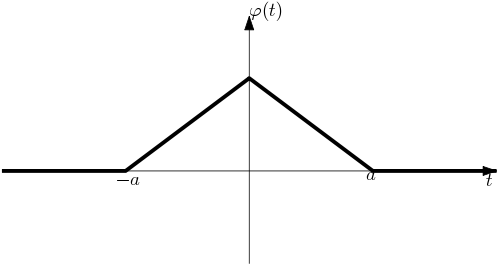
\includegraphics[scale=0.4]{img/img1.png}
		\end{center}
		является характеристической.
	\end{example}

	\begin{theorem}[Марцинкевича(б/д)]
		Если характеристическая функция \(\varphi(t)\) имеет вид ~\(\exp(P(t)),\) где \(P(t)\)~--- полином, то степерь этого полинома \(\leqslant 2 ~(\deg P(t) \leqslant 2).\)
	\end{theorem}
	\begin{example}
		\(e^{-t^n}\) не является характеристической функцией.
	\end{example}

	\begin{definition}
		Последовательность функций \(F_n(x)\) слабо сходится к \(F(x)\), если \(\forall f(x)\)~---  непрерывна и ограничена, то верно \(\int\limits_\R f(x) df_n(x) \to \int\limits_\R f(x)dF(x).\) Обозначение \(F_n \overset{w}{\longrightarrow}F.\)
		\((\xi_n \overset{d}{\longrightarrow}\xi \Leftrightarrow F_{\xi_n} \overset{w}{\longrightarrow}F).\)
	\end{definition}
	\begin{theorem}[нерперывности для х.ф.]~~~~~~~~~~~~~~~~~~~~~~~~~~~~~~~~~~~~~~~~~

		\noindent1. ~Пусть \(\{F_n\}_{n \geqslant 1}\)~--- последовательность функций распределения на \(\R\), тогда \(\varphi_n(t) \to \varphi(t) ~ \forall t \in \R, \) где \(\varphi\)~--- характеристическая функция \(F\).
		
		\noindent2.(б/д)~ Пусть \(\forall t \in \R ~ \exists \varphi(t) = \lim\limits_{n \to +\infty} \varphi_n(t), \) причём \(\varphi(t)\) непрерывна в нуле. Тогда \(\exists F\)~--- функция распределения такая, что \(F_n \overset{w}{\longrightarrow}F\) и \(\varphi\)~---характеристическая функция \(F\).
	\end{theorem}

	\begin{proof}
		Знаем, что  \(\forall f\)~--- непрерывной ограниченной функции : \(\int\limits_\R f(x)dF_n(x) \to \int\limits_\R f(x)dF(x).\) Но функции \(\sin tx \) и \(\cos tx\) непрерывны и ограничены \(\Rightarrow\) \(\varphi_n(t) = \int\limits_\R (\cos tx + i\sin tx)dF_n(x) \underset{n \to +\infty}{\longrightarrow} \int\limits_\R (\cos tx + i\sin tx)dF(x) = \varphi(t).\)
	\end{proof}

	\subsection{Центральная предельная теорема}
	\begin{theorem}[ЦПТ в форме Леви]
		Пусть \(\{\xi_n\}_{n\geqslant 1}\)~--- независимые одинаково распределённые случайные величины, \(0 < D\xi < +\infty.\)
		Обозначим \(S_n = \sum\limits_{i = 1}^{n}\xi_i.\) Тогда 
		\(\frac{S_n - ES_n}{\sqrt{DS_n}} \overset{d}{\underset{n \to +\infty}{\longrightarrow}}N(0, 1).\)
	\end{theorem}

	\begin{proof}
		Обозначим \(E\xi_i = a, D\xi_i = \sigma^2.\)
		Рассмотрим случайные величины \(\eta_i = \frac{\xi_i - a}{\sigma} \Rightarrow 
		E\eta_i = 0; ~ D\eta_i = 1.\)
		Тогда \(T_n = \frac{S_n - ES_n}{\sqrt{DS_n}} = \frac{S_n - na}{\sqrt{n\sigma^2}} = \frac{\eta_1 + \ldots + \eta_n}{\sqrt{n}}.\)
		Рассмотрим характеристическую функцию \(\eta_i\): по свойствам характеристической функции \(\varphi(t) \equiv \varphi_{\eta_i}(t) = 1 + it\underbracket{E\eta_j}_{0} + \frac{1}{2}\underbracket{E\eta_j^2}_1\cdot(it)^2 + o(t^2 = 1 - \frac{t^2}{2} + o(t^2), ~ t \to 0.\) Отсюда, \(\varphi_{T_n}(t) = \varphi_{\sum\limits_{j = 1}^{n}\eta_j}(t) \overset{\text{св-ва х.ф.}}{=} \left(\varphi\left(\frac{t}{\sqrt{n}}\right)\right)^n = \left(1 - \frac{t^2}{2} + o\left(\frac{t^2}{n}\right)\right)^n \underset{n \to \infty}{=} e^{- \frac{t^2}{2}}. \)Но \(e^{-\frac{t^2}{2}}\)~--- характеристическая функция \(N(0,1) \Rightarrow\) (по т. непрерывности) \(T_n = \frac{S_n - ES_n}{\sqrt{DS_n}} \overset{d}{\longrightarrow} N(0,1).\)
	\end{proof}